\documentclass[aspectratio=169,10pt]{ctexbeamer}
\usetheme{default}
\usefonttheme{professionalfonts}
\usepackage{amsmath,amssymb,mathtools,bm,braket}
\usepackage{booktabs,array,multirow}
\usepackage{tikz}
\usetikzlibrary{arrows.meta,positioning,calc,decorations.pathreplacing,shapes.geometric,fit,backgrounds}
\usepackage{quantikz}
\usepackage[most]{tcolorbox}
\usepackage{physics}
\usepackage{hyperref}

% --- Colors: modeled after the uploaded PDE quantum foundations slides ---
\definecolor{navy}{RGB}{0,0,145}
\definecolor{deepred}{RGB}{150,0,0}
\definecolor{softblue}{RGB}{238,242,255}
\definecolor{softred}{RGB}{255,238,238}
\definecolor{softgreen}{RGB}{238,250,238}
\definecolor{softyellow}{RGB}{255,248,225}
\definecolor{darkgreen}{RGB}{30,105,50}
\definecolor{graytext}{RGB}{70,70,70}

\setbeamercolor{frametitle}{fg=white,bg=navy}
\setbeamerfont{frametitle}{series=\bfseries,size=\large}
\setbeamercolor{title}{fg=black,bg=white}
\setbeamercolor{structure}{fg=navy}
\setbeamercolor{block title}{fg=white,bg=navy}
\setbeamercolor{block body}{fg=black,bg=softblue}
\setbeamercolor{alerted text}{fg=deepred}
\setbeamertemplate{navigation symbols}{}
\setbeamertemplate{itemize item}{\color{navy}$\blacktriangleright$}
\setbeamertemplate{itemize subitem}{\color{navy}$\triangleright$}
\setbeamertemplate{enumerate item}{\color{navy}\insertenumlabel.}
\setbeamertemplate{frametitle}{%
  \nointerlineskip
  \begin{beamercolorbox}[wd=\paperwidth,ht=2.9ex,dp=0.9ex,leftskip=1.0em]{frametitle}
    \insertframetitle
  \end{beamercolorbox}}
\setbeamertemplate{footline}{%
  \hfill\scriptsize\color{graytext}\insertframenumber{} / \inserttotalframenumber\hspace{1.5em}\vspace{0.7em}}

\newtcolorbox{keybox}[1]{colback=softblue,colframe=navy,title={#1},fonttitle=\bfseries,boxrule=0.6pt,arc=1.5mm,left=1.5mm,right=1.5mm,top=1mm,bottom=1mm}
\newtcolorbox{warnbox}[1]{colback=softred,colframe=deepred,title={#1},fonttitle=\bfseries,boxrule=0.6pt,arc=1.5mm,left=1.5mm,right=1.5mm,top=1mm,bottom=1mm}
\newtcolorbox{exbox}[1]{colback=softyellow,colframe=darkgreen,title={#1},fonttitle=\bfseries,boxrule=0.6pt,arc=1.5mm,left=1.5mm,right=1.5mm,top=1mm,bottom=1mm}
\newcommand{\C}{\mathbb{C}}
\newcommand{\R}{\mathbb{R}}
\newcommand{\N}{\mathbb{N}}
\newcommand{\eps}{\varepsilon}
\newcommand{\poly}{\operatorname{poly}}
\newcommand{\argmin}{\operatorname*{argmin}}
\newcommand{\ii}{\mathrm{i}}
\newcommand{\e}{\mathrm{e}}
\newcommand{\ketzero}{\ket{0}}
\newcommand{\ketone}{\ket{1}}
\newcommand{\ketplus}{\ket{+}}
\newcommand{\ketminus}{\ket{-}}
\newcommand{\smallcite}[1]{\par\vspace{1mm}{\scriptsize\color{graytext}#1}}

\title{Quantum Computation Basics\vspace{1mm}\\\large 面向数学专业学生的量子计算基础课件}
\author{基于上传 PDF 内容整理与扩展}
\date{\today}

\begin{document}

% -------------------------------------------------------------------
\begin{frame}[plain]
\vspace{1.5cm}
{\LARGE\bfseries Quantum Computation Basics}\par\vspace{3mm}
{\large 面向数学专业学生的量子计算基础}\par\vspace{8mm}
\begin{tikzpicture}[scale=0.95]
  \node[draw=navy,rounded corners,thick,fill=softblue,minimum width=2.7cm,minimum height=0.75cm] (h) {Hilbert 空间};
  \node[draw=navy,rounded corners,thick,fill=softblue,minimum width=2.7cm,minimum height=0.75cm,right=1.0cm of h] (u) {酉线路};
  \node[draw=navy,rounded corners,thick,fill=softblue,minimum width=2.7cm,minimum height=0.75cm,right=1.0cm of u] (m) {测量与采样};
  \node[draw=navy,rounded corners,thick,fill=softblue,minimum width=2.7cm,minimum height=0.75cm,right=1.0cm of m] (a) {QFT/QPE};
  \draw[-Latex,thick] (h)--(u); \draw[-Latex,thick] (u)--(m); \draw[-Latex,thick] (m)--(a);
\end{tikzpicture}
\vfill
{\small 讲义式、公式推导式、面向 PDE 与科学计算量子算法的第一课}
\end{frame}

\begin{frame}{从 PDE 到量子算法：本课处在什么位置？}
\begin{center}
\begin{tikzpicture}[node distance=7mm, every node/.style={font=\small,align=center}]
\node[draw,rounded corners,fill=white,minimum width=2.2cm,minimum height=0.8cm] (pde) {连续 PDE\\$u_t=Lu$};
\node[draw,rounded corners,fill=softgreen,minimum width=2.2cm,minimum height=0.8cm,right=of pde] (disc) {离散化\\$A_h,H_h$};
\node[draw,rounded corners,fill=softyellow,minimum width=2.2cm,minimum height=0.8cm,right=of disc] (enc) {量子编码\\ $\ket{u_h}$};
\node[draw,rounded corners,fill=softred,minimum width=2.2cm,minimum height=0.8cm,right=of enc] (alg) {量子变换\\QFT/QPE/HS};
\node[draw,rounded corners,fill=white,minimum width=2.2cm,minimum height=0.8cm,right=of alg] (out) {读出结果\\观测量/样本};
\draw[-Latex,thick] (pde)--(disc); \draw[-Latex,thick] (disc)--(enc); \draw[-Latex,thick] (enc)--(alg); \draw[-Latex,thick] (alg)--(out);
\end{tikzpicture}
\end{center}
\begin{keybox}{第 1 课目标}
先把量子态、酉演化、量子线路、测量、采样误差、复杂度模型讲清楚；然后以 QFT/QPE 为桥梁，说明量子算法如何接入 Fourier 谱方法与 PDE 问题。
\end{keybox}
\end{frame}

\begin{frame}{本课知识地图}
\begin{columns}[T,totalwidth=\textwidth]
\column{0.49\textwidth}
\begin{keybox}{数学基础}
\begin{itemize}
\item Hilbert 空间、Dirac 符号、张量积
\item 谱分解、SVD、矩阵函数
\item 量子态、酉矩阵、可观测量、密度矩阵
\end{itemize}
\end{keybox}
\begin{keybox}{线路与测量}
\begin{itemize}
\item 常用门：$X,Y,Z,H,S,T,R_z$, CNOT, Toffoli
\item 受控酉、可逆计算、Hadamard/SWAP test
\item shots、postselection、误差传播
\end{itemize}
\end{keybox}
\column{0.49\textwidth}
\begin{keybox}{算法接口}
\begin{itemize}
\item 量子复杂度：qubits/gates/queries/shots
\item 稀疏矩阵与 Hamiltonian 表示
\item QFT、QPE、相位回踢
\end{itemize}
\end{keybox}
\begin{keybox}{面向科学计算的观点}
\begin{itemize}
\item 输入与输出瓶颈决定可否加速
\item PDE 离散矩阵必须能被线路有效访问
\item 量子输出通常是态或观测量，而非全量数组
\end{itemize}
\end{keybox}
\end{columns}
\end{frame}

\section{计算模型与量子优势}

\begin{frame}{本课程默认的计算模型：FTQC}
\begin{center}
\begin{tikzpicture}[node distance=9mm, every node/.style={font=\small,align=center}]
\node[draw,rounded corners,fill=softred,minimum width=2.3cm,minimum height=0.85cm] (p) {物理量子比特\\physical qubits};
\node[draw,rounded corners,fill=softblue,minimum width=2.3cm,minimum height=0.85cm,right=of p] (ec) {量子纠错\\syndrome};
\node[draw,rounded corners,fill=softgreen,minimum width=2.3cm,minimum height=0.85cm,right=of ec] (l) {逻辑量子比特\\logical qubits};
\node[draw,rounded corners,fill=softyellow,minimum width=2.3cm,minimum height=0.85cm,right=of l] (alg) {算法层\\queries/shots};
\draw[-Latex,thick] (p)--(ec); \draw[-Latex,thick] (ec)--(l); \draw[-Latex,thick] (l)--(alg);
\end{tikzpicture}
\end{center}
\begin{keybox}{Fully fault-tolerant quantum computer}
容错量子计算假设物理噪声已由量子纠错压低到逻辑层。算法分析主要统计逻辑门数、查询次数、辅助量子比特数、测量次数与数学近似误差。
\end{keybox}
\begin{warnbox}{为什么不是只讲 NISQ？}
QFT、QPE、HHL、Hamiltonian simulation、QSVT 等科学计算算法通常需要深线路与高精度，因此更自然地放在 FTQC 框架中分析。
\end{warnbox}
\end{frame}

\begin{frame}{NISQ 与 FTQC：两类问题意识}
\begin{center}
\renewcommand{\arraystretch}{1.15}
\begin{tabular}{p{0.19\textwidth}p{0.33\textwidth}p{0.33\textwidth}}
\toprule
& \textbf{NISQ 设备} & \textbf{FTQC 设备}\\
\midrule
量子比特 & 物理比特数量有限，噪声显著 & 逻辑比特由纠错码保护\\
线路深度 & 不能太深 & 可执行长线路\\
典型算法 & VQE、QAOA、误差缓解 & QFT、QPE、HHL、Hamiltonian simulation\\
数学分析 & 经验性能、噪声适应 & 渐近复杂度、误差界、可证明加速\\
本课定位 & 背景了解 & 默认模型\\
\bottomrule
\end{tabular}
\end{center}
\vspace{2mm}
\begin{keybox}{科学计算中的核心问题}
量子计算不是“把矩阵丢给量子计算机”。必须说明：数据如何编码、矩阵如何访问、输出如何读取、误差如何累积、与最强经典 baseline 如何比较。
\end{keybox}
\end{frame}

\begin{frame}{量子优势不是“叠加态 = 自动加速”}
\begin{columns}[T,totalwidth=\textwidth]
\column{0.56\textwidth}
$n$ 个量子比特的态空间维数是 $2^n$，但测量只能给出一个 bit string。宣称加速前至少要问：
\begin{enumerate}
\item 是否需要指数规模的经典输入？
\item 是否要求读出指数规模的经典输出？
\item 经典算法是否真的必须遍历全部状态？
\item 当前经典算法慢，是否因为还没有更好的算法？
\end{enumerate}
\column{0.42\textwidth}
\begin{tikzpicture}[scale=0.9,every node/.style={font=\small,align=center}]
\node[draw,rounded corners,fill=softblue,align=center,minimum width=3.3cm,minimum height=0.85cm] (state) {指数维态空间\\ $\sum_x \alpha_x\ket{x}$};
\node[draw,rounded corners,fill=softred,align=center,below=0.9cm of state,minimum width=3.3cm,minimum height=0.85cm] (meas) {一次测量\\得到一个 $x$};
\draw[-Latex,thick] (state)--node[right]{Born 规则} (meas);
\node[draw,rounded corners,fill=softyellow,align=center,below=0.9cm of meas,minimum width=3.3cm,minimum height=0.85cm] (obs) {可行输出\\样本/期望值/少量特征};
\draw[-Latex,thick] (meas)--(obs);
\end{tikzpicture}
\end{columns}
\smallcite{Feynman 关于量子模拟的早期动机见 R. P. Feynman, Int. J. Theor. Phys. 21, 467--488 (1982).}
\end{frame}

\begin{frame}{怎样度量量子加速？}
\begin{keybox}{一个有用的粗略定义}
令系统规模为 $n$，经典最优代价为 $C_{\rm cl}(n)$，量子代价为 $C_{\rm q}(n)$，可用
\[
\text{speedup ratio} = \frac{\log C_{\rm cl}(n)}{\log C_{\rm q}(n)}
\]
粗略区分二次、三次、超多项式和指数加速。
\end{keybox}
\begin{columns}[T,totalwidth=\textwidth]
\column{0.5\textwidth}
\begin{exbox}{例：Grover 搜索}
非结构搜索：经典查询 $\Theta(N)$，量子查询 $\Theta(\sqrt N)$。这是可证明最优的二次加速。
\end{exbox}
\column{0.5\textwidth}
\begin{exbox}{例：Shor 分解}
输入长度 $n=\log_2 M$。Shor 算法给出多项式时间量子算法；当前最好经典算法为亚指数复杂度。
\end{exbox}
\end{columns}
\end{frame}

\begin{frame}{科学计算中的量子算法评估框架}
\begin{center}
\begin{tikzpicture}[node distance=8mm, every node/.style={font=\small,align=center}]
\node[draw,rounded corners,fill=softblue,minimum width=2.7cm,minimum height=0.8cm] (input) {输入模型\\oracle / state prep};
\node[draw,rounded corners,fill=softgreen,right=of input,minimum width=2.7cm,minimum height=0.8cm] (transform) {矩阵变换\\unitary / block-encoding};
\node[draw,rounded corners,fill=softyellow,right=of transform,minimum width=2.7cm,minimum height=0.8cm] (measure) {测量读出\\samples / observables};
\node[draw,rounded corners,fill=softred,right=of measure,minimum width=2.7cm,minimum height=0.8cm] (compare) {经典比较\\baseline};
\draw[-Latex,thick] (input)--(transform); \draw[-Latex,thick] (transform)--(measure); \draw[-Latex,thick] (measure)--(compare);
\end{tikzpicture}
\end{center}
\begin{warnbox}{数学专业学生需要特别注意}
量子算法的“输入”和“输出”通常不是普通数组。若要加载完整 $N$ 维向量或读出全部 $N$ 个分量，潜在指数优势会被输入/输出成本抵消。
\end{warnbox}
\end{frame}

\section{Hilbert 空间与量子力学公设}

\begin{frame}{两个维数：$n$ 与 $N=2^n$}
\begin{columns}[T,totalwidth=\textwidth]
\column{0.52\textwidth}
\begin{keybox}{量子信息的维数账本}
\begin{itemize}
\item $n$：量子比特数。
\item $N=2^n$：计算基态数量，也就是 Hilbert 空间维数。
\item 经典 $n$ bit 只处在一个字符串 $x\in\{0,1\}^n$。
\item 量子 $n$ qubit 可以处在 $N$ 维复向量空间中的单位向量。
\end{itemize}
\end{keybox}
\column{0.45\textwidth}
\[
\ket{\psi}=\sum_{x\in\{0,1\}^n}\alpha_x\ket{x},
\quad \sum_x |\alpha_x|^2=1.
\]
\begin{exbox}{例}
$n=3$ 时 $N=8$，基态为 $\ket{000},\ket{001},\ldots,\ket{111}$。
\end{exbox}
\end{columns}
\end{frame}

\begin{frame}{计算基与 bit string}
$n$ 个 qubit 的计算基由所有二进制串给出：
\[
\{\ket{x}:x\in\{0,1\}^n\}.
\]
若
\[
x=(x_{n-1}\cdots x_1x_0)_2,\qquad j=\sum_{r=0}^{n-1}x_r2^r,
\]
则常把
\[
\ket{x}=\ket{x_{n-1}}\otimes\cdots\otimes\ket{x_0}
\]
也写作 $\ket{j}$。
\begin{exbox}{例}
$3$ 个 qubit 中 $j=5=(101)_2$，故 $\ket{5}=\ket{101}$。
\end{exbox}
\begin{warnbox}{约定提醒}
不同教材或软件框架可能采用不同端序。量子线路推导中必须固定 bit order，否则 QFT 与相位读出会出现翻转。
\end{warnbox}
\end{frame}

\begin{frame}{Dirac 符号：ket、bra、内积与外积}
\begin{columns}[T,totalwidth=\textwidth]
\column{0.5\textwidth}
\begin{keybox}{向量与对偶向量}
\[
\ket{\psi}=\begin{pmatrix}\alpha_0\\ \alpha_1\\ \vdots\end{pmatrix},
\qquad
\bra{\psi}=\ket{\psi}^{\dagger}=(\overline{\alpha_0},\overline{\alpha_1},\ldots).
\]
内积写作
\[
\braket{\phi|\psi}=\bra{\phi}\ket{\psi}.
\]
\end{keybox}
\column{0.5\textwidth}
\begin{keybox}{投影与秩一算子}
\[
\ket{\psi}\bra{\phi}: v\mapsto \ket{\psi}\braket{\phi|v}.
\]
特别地，若 $\|\psi\|=1$，则
\[
P_{\psi}=\ket{\psi}\bra{\psi},\quad P_{\psi}^2=P_{\psi}=P_{\psi}^{\dagger}.
\]
\end{keybox}
\end{columns}
\end{frame}

\begin{frame}{公设 1：量子态是单位向量}
\begin{keybox}{态空间公设}
孤立量子系统由复 Hilbert 空间 $\mathcal H$ 描述。纯态是单位向量 $\ket{\psi}\in\mathcal H$，相差全局相位的向量表示同一物理态：
\[
\ket{\psi}\sim e^{i\theta}\ket{\psi}.
\]
\end{keybox}
\begin{columns}[T,totalwidth=\textwidth]
\column{0.55\textwidth}
单 qubit 一般纯态写作
\[
\ket{\psi}=\alpha\ket{0}+\beta\ket{1},\quad |\alpha|^2+|\beta|^2=1.
\]
\column{0.4\textwidth}
去掉全局相位后也可写为
\[
\ket{\psi}=\cos\frac\theta2\ket{0}+e^{i\varphi}\sin\frac\theta2\ket{1}.
\]
\end{columns}
\end{frame}

\begin{frame}{Bloch 球：单 qubit 的几何图像}
\begin{columns}[T,totalwidth=\textwidth]
\column{0.48\textwidth}
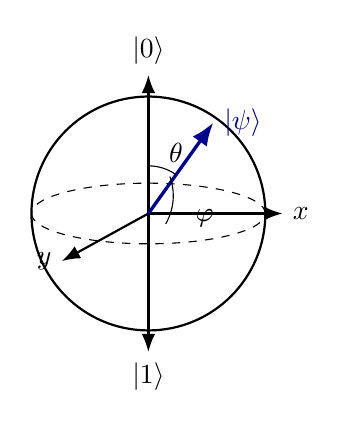
\begin{tikzpicture}[scale=1.1]
\draw[thick] (0,0) circle (1.35);
\draw[dashed] (-1.35,0) arc (180:360:1.35 and 0.35);
\draw[dashed] (1.35,0) arc (0:180:1.35 and 0.35);
\draw[-Latex,thick] (0,0)--(0,1.6) node[above] {$\ket{0}$};
\draw[-Latex,thick] (0,0)--(0,-1.6) node[below] {$\ket{1}$};
\draw[-Latex,thick] (0,0)--(1.55,0) node[right] {$x$};
\draw[-Latex,thick] (0,0)--(-1.0,-0.55) node[left] {$y$};
\draw[-Latex,very thick,navy] (0,0)--(0.75,1.05) node[right] {$\ket{\psi}$};
\draw (0,0.55) arc (90:55:0.55); \node at (0.32,0.70) {$\theta$};
\draw (0.2,-0.12) arc (-30:20:0.65); \node at (0.65,-0.05) {$\varphi$};
\end{tikzpicture}
\column{0.50\textwidth}
\begin{keybox}{参数化}
\[
\ket{\psi}=\cos\frac\theta2\ket{0}+e^{i\varphi}\sin\frac\theta2\ket{1}.
\]
\[
\rho=\ket{\psi}\bra{\psi}=\frac12(I+\bm r\cdot\bm\sigma),\quad \|\bm r\|=1.
\]
\end{keybox}
\begin{warnbox}{局限}
Bloch 球只完整描述单 qubit 纯态。多 qubit 态空间维数指数增长，不能用一个三维球直观表示。
\end{warnbox}
\end{columns}
\end{frame}

\begin{frame}{公设 2：封闭系统演化是酉的}
\begin{keybox}{演化公设}
封闭量子系统从时刻 $t_1$ 到 $t_2$ 的演化由酉矩阵 $U$ 给出：
\[
\ket{\psi(t_2)}=U\ket{\psi(t_1)},\qquad U^{\dagger}U=I.
\]
酉性保证范数与内积不变：
\[
\|U\psi\|=\|\psi\|,\qquad \braket{U\phi|U\psi}=\braket{\phi|\psi}.
\]
\end{keybox}
\begin{exbox}{数学理解}
量子线路中的每个门都是一个低维酉矩阵；把它嵌入大 Hilbert 空间后，相乘得到整体酉矩阵。
\end{exbox}
\end{frame}

\begin{frame}{Hamiltonian 与 Schr\"odinger 方程}
连续时间演化由 Hermitian 算子 $H=H^{\dagger}$ 生成：
\[
 i\frac{d}{dt}\ket{\psi(t)}=H\ket{\psi(t)}.
\]
若 $H$ 与时间无关，则
\[
\ket{\psi(t)}=e^{-iHt}\ket{\psi(0)},\qquad U(t)=e^{-iHt}\text{ 是酉矩阵}.
\]
\begin{keybox}{与矩阵函数的联系}
若 $H=\sum_j \lambda_j\ket{v_j}\bra{v_j}$，则
\[
 e^{-iHt}=\sum_j e^{-i\lambda_jt}\ket{v_j}\bra{v_j}.
\]
所以 Hamiltonian simulation 本质上是高效实现矩阵函数 $f(H)=e^{-iHt}$。
\end{keybox}
\end{frame}

\begin{frame}{常用单 qubit 门}
\begin{center}
\renewcommand{\arraystretch}{1.35}
\begin{tabular}{c c c}
\toprule
门 & 矩阵 & 作用\\
\midrule
$X$ & $\begin{pmatrix}0&1\\1&0\end{pmatrix}$ & bit flip：$\ket0\leftrightarrow\ket1$\\
$Z$ & $\begin{pmatrix}1&0\\0&-1\end{pmatrix}$ & phase flip：$\ket1\mapsto-\ket1$\\
$H$ & $\frac1{\sqrt2}\begin{pmatrix}1&1\\1&-1\end{pmatrix}$ & 产生/消除叠加，Fourier on $\mathbb Z_2$\\
$S$ & $\begin{pmatrix}1&0\\0&i\end{pmatrix}$ & $\pi/2$ 相位\\
$T$ & $\begin{pmatrix}1&0\\0&e^{i\pi/4}\end{pmatrix}$ & 非 Clifford 相位\\
$R_z(\theta)$ & $e^{-i\theta Z/2}$ & $z$ 轴旋转\\
\bottomrule
\end{tabular}
\end{center}
\end{frame}

\begin{frame}{公设 3：测量与 Born 规则}
\begin{keybox}{计算基测量}
对
\[
\ket{\psi}=\sum_{x\in\{0,1\}^n}\alpha_x\ket{x},
\]
在计算基测量得到 $x$ 的概率为
\[
\Pr[x]=|\alpha_x|^2.
\]
测量后状态坍缩为对应的 $\ket{x}$。
\end{keybox}
\begin{warnbox}{重要后果}
叠加态的全部振幅不能由一次测量读出。量子算法通常通过干涉把目标信息转化为某些测量概率或少量 bit string 的高概率事件。
\end{warnbox}
\end{frame}

\begin{frame}{一般投影测量与期望值}
可观测量 $M=M^{\dagger}$ 有谱分解
\[
M=\sum_m \lambda_m P_m.
\]
对态 $\ket\psi$ 测量得到 $\lambda_m$ 的概率为
\[
p_m=\bra\psi P_m\ket\psi,
\]
测量后的状态为
\[
\ket\psi\mapsto \frac{P_m\ket\psi}{\sqrt{p_m}}.
\]
期望值为
\[
\mathbb E_{\psi}(M)=\sum_m\lambda_m p_m=\bra\psi M\ket\psi.
\]
\begin{exbox}{科学计算接口}
许多 PDE 量子算法最终估计的是 $\bra{u}M\ket{u}$，例如能量、质量、内积或局部平均量。
\end{exbox}
\end{frame}

\begin{frame}{公设 4：复合系统与张量积}
若系统 $A$ 的 Hilbert 空间为 $\mathcal H_A$，系统 $B$ 为 $\mathcal H_B$，则复合系统为
\[
\mathcal H_{AB}=\mathcal H_A\otimes\mathcal H_B.
\]
若
\[
\ket\phi=\sum_i a_i\ket{i},\qquad \ket\psi=\sum_j b_j\ket{j},
\]
则
\[
\ket\phi\otimes\ket\psi=\sum_{i,j}a_i b_j\ket{i}\ket{j}.
\]
\begin{keybox}{维数指数增长}
$n$ 个 qubit 的空间是 $(\mathbb C^2)^{\otimes n}\cong\mathbb C^{2^n}$。
这既是量子计算潜力来源，也是经典模拟困难来源。
\end{keybox}
\end{frame}

\begin{frame}{纠缠：张量积空间中并非都是直积态}
\begin{columns}[T,totalwidth=\textwidth]
\column{0.48\textwidth}
Bell 态
\[
\ket{\Phi^+}=\frac{\ket{00}+\ket{11}}{\sqrt2}
\]
不能写成 $\ket a\otimes\ket b$。
\begin{exbox}{证明思路}
若 $(\alpha\ket0+\beta\ket1)\otimes(\gamma\ket0+\delta\ket1)$ 等于 Bell 态，则需
\[
\alpha\gamma=\frac1{\sqrt2},\; \beta\delta=\frac1{\sqrt2},\; \alpha\delta=0,
\; \beta\gamma=0,
\]
矛盾。
\end{exbox}
\column{0.5\textwidth}
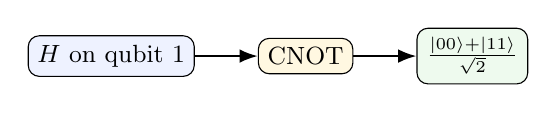
\begin{tikzpicture}[node distance=8mm, every node/.style={font=\small,align=center}]
\node[draw,rounded corners,fill=softblue] (h) {$H$ on qubit 1};
\node[draw,rounded corners,fill=softyellow,right=of h] (c) {CNOT};
\node[draw,rounded corners,fill=softgreen,right=of c] (b) {$\frac{\ket{00}+\ket{11}}{\sqrt2}$};
\draw[-Latex,thick] (h)--(c); \draw[-Latex,thick] (c)--(b);
\end{tikzpicture}
\vspace{3mm}
\[
\ket{00}\xrightarrow{H\otimes I}\frac{\ket{00}+\ket{10}}{\sqrt2}
\xrightarrow{\mathrm{CNOT}}\frac{\ket{00}+\ket{11}}{\sqrt2}.
\]
\end{columns}
\end{frame}


\begin{frame}{No-cloning theorem：未知量子态不能复制}
\small
\begin{keybox}{命题}
不存在酉矩阵 $U$，使得对所有未知态 $\ket\psi$ 都有
\[
U\ket\psi\ket0=\ket\psi\ket\psi.
\]
\end{keybox}
\begin{keybox}{证明：酉性保持内积}
若对任意 $\ket\psi,\ket\phi$ 都能复制，则
\[
U\ket\psi\ket0=\ket\psi\ket\psi,
\qquad
U\ket\phi\ket0=\ket\phi\ket\phi.
\]
两边取内积并利用 $U^{\dagger}U=I$，得到
\[
\braket{\psi|\phi}=\braket{\psi|\phi}^2.
\]
因此只能有 $\braket{\psi|\phi}=0$ 或 $1$，与任意非正交未知态矛盾。
\end{keybox}
\begin{warnbox}{算法后果}
量子数据不能随意复制；很多线路必须使用可逆计算与 uncompute 清除垃圾态。
\end{warnbox}
\end{frame}

\begin{frame}{密度算子：纯态、混合态与子系统}
\begin{columns}[T,totalwidth=\textwidth]
\column{0.49\textwidth}
\begin{keybox}{纯态}
\[
\rho=\ket\psi\bra\psi,
\qquad \rho^2=\rho,
\quad \mathrm{Tr}(\rho)=1.
\]
\end{keybox}
\begin{keybox}{混合态}
若以概率 $p_j$ 制备 $\ket{\psi_j}$，则
\[
\rho=\sum_j p_j\ket{\psi_j}\bra{\psi_j}.
\]
\end{keybox}
\column{0.49\textwidth}
\begin{keybox}{部分迹}
复合系统 $AB$ 中，只看 $A$ 的状态：
\[
\rho_A=\mathrm{Tr}_B(\rho_{AB}).
\]
\end{keybox}
\begin{exbox}{Bell 态的子系统}
对 $\ket{\Phi^+}$，有
\[
\rho_A=\frac12 I.
\]
整体是纯态，局部却是完全混合态。
\end{exbox}
\end{columns}
\end{frame}

\section{量子线路与可逆计算}

\begin{frame}{量子线路语言：线、门、控制与测量}
\begin{center}
\begin{quantikz}[row sep=0.28cm,column sep=0.45cm]
\lstick{$\ket{0}$} & \gate{H} & \ctrl{1} & \gate{R_z(\theta)} & \meter{} \\
\lstick{$\ket{0}$} & \qw      & \targ{}  & \qw             & \meter{}
\end{quantikz}
\end{center}
\begin{keybox}{读线路的顺序}
\begin{itemize}
\item 每条线表示一个 qubit；时间通常从左到右。
\item 一个门作用在对应的 qubit 子空间，并隐含与其余 qubit 的恒等张量积。
\item 控制门是分块酉矩阵：控制位为 $0$ 不动，控制位为 $1$ 时作用目标酉。
\item 测量通常放在线路末端；若中途测量，需要说明经典反馈。
\end{itemize}
\end{keybox}
\end{frame}

\begin{frame}{受控酉门与 CNOT}
\begin{columns}[T,totalwidth=\textwidth]
\column{0.48\textwidth}
\begin{center}
\begin{quantikz}[row sep=0.35cm,column sep=0.5cm]
\lstick{$\ket c$} & \ctrl{1} & \qw \\
\lstick{$\ket b$} & \targ{} & \qw
\end{quantikz}
\end{center}
\[
\mathrm{CNOT}\ket{c,b}=\ket{c,b\oplus c}.
\]
矩阵为
\[
\begin{pmatrix}
1&0&0&0\\0&1&0&0\\0&0&0&1\\0&0&1&0
\end{pmatrix}.
\]
\column{0.50\textwidth}
\begin{center}
\begin{quantikz}[row sep=0.35cm,column sep=0.5cm]
\lstick{$\ket c$} & \ctrl{1} & \qw \\
\lstick{$\ket \psi$} & \gate{U} & \qw
\end{quantikz}
\end{center}
\[
C(U)=\ket0\bra0\otimes I+\ket1\bra1\otimes U.
\]
\begin{exbox}{相位回踢的入口}
若目标态是 $U$ 的本征态，控制寄存器会获得对应本征相位。这是 QPE 的关键。
\end{exbox}
\end{columns}
\end{frame}

\begin{frame}{通用门集：连续数学到离散线路}
\begin{keybox}{精确通用与近似通用}
一个门集若能以任意精度逼近任意 $n$ qubit 酉矩阵，称为通用门集。常见容错门集：
\[
\{H,S,T,\mathrm{CNOT}\}.
\]
其中 Clifford 门 $\{H,S,\mathrm{CNOT}\}$ 容易经典模拟；$T$ 门提供非 Clifford 资源。
\end{keybox}
\begin{columns}[T,totalwidth=\textwidth]
\column{0.5\textwidth}
\begin{exbox}{数学上}
任意 $U\in U(2^n)$ 可分解为若干两能级酉矩阵，再分解为单比特旋转和 CNOT。
\end{exbox}
\column{0.5\textwidth}
\begin{warnbox}{算法上}
论文中的“一个受控 $e^{-iHt}$”在真实成本中必须分解成基本逻辑门，并计入近似误差。
\end{warnbox}
\end{columns}
\end{frame}

\begin{frame}{经典可逆计算：为什么量子线路需要 uncompute？}
经典不可逆门如 AND 会丢失信息：
\[
(a,b)\mapsto a\land b.
\]
量子封闭演化必须可逆，因此通常使用 Toffoli 门实现
\[
\ket{a,b,c}\mapsto \ket{a,b,c\oplus ab}.
\]
\begin{center}
\begin{quantikz}[row sep=0.28cm,column sep=0.48cm]
\lstick{$\ket a$} & \ctrl{2} & \qw \\
\lstick{$\ket b$} & \ctrl{1} & \qw \\
\lstick{$\ket c$} & \targ{}  & \qw
\end{quantikz}
\end{center}
\begin{keybox}{compute - use - uncompute}
若计算 $f(x)$ 只为控制后续操作，常用
\[
\ket{x}\ket0 \xrightarrow{U_f} \ket{x}\ket{f(x)} \xrightarrow{\text{use}} \cdots \xrightarrow{U_f^{\dagger}} \ket{x}\ket0
\]
把辅助寄存器还原，避免垃圾态与主系统纠缠。
\end{keybox}
\end{frame}

\begin{frame}{量子数据编码：basis、amplitude 与 oracle}
\begin{columns}[T,totalwidth=\textwidth]
\column{0.32\textwidth}
\begin{keybox}{Basis encoding}
\[
x\in\{0,1\}^n\mapsto\ket{x}.
\]
适合组合、索引、离散状态。
\end{keybox}
\column{0.32\textwidth}
\begin{keybox}{Amplitude encoding}
\[
u\in\mathbb C^N\mapsto\ket u=\frac{1}{\|u\|}\sum_j u_j\ket j.
\]
适合数值线性代数，但制备成本必须说明。
\end{keybox}
\column{0.32\textwidth}
\begin{keybox}{Oracle access}
\[
O_f\ket{x}\ket{y}=\ket{x}\ket{y\oplus f(x)}.
\]
适合黑盒函数、稀疏矩阵或 PDE 规则访问。
\end{keybox}
\end{columns}
\vspace{2mm}
\begin{warnbox}{关键限制}
Amplitude encoding 把 $N$ 个数压进 $\log N$ 个 qubit，但不意味着可以免费装载或完整读出 $N$ 个数。
\end{warnbox}
\end{frame}

\begin{frame}{PDE 网格函数的 amplitude encoding}
设一维网格有 $N=2^n$ 个点，网格函数为
\[
\bm u=(u_0,u_1,\ldots,u_{N-1})^T\in\mathbb C^N.
\]
量子态编码为
\[
\ket u=\frac{1}{\|\bm u\|_2}\sum_{j=0}^{N-1}u_j\ket j.
\]
\begin{center}
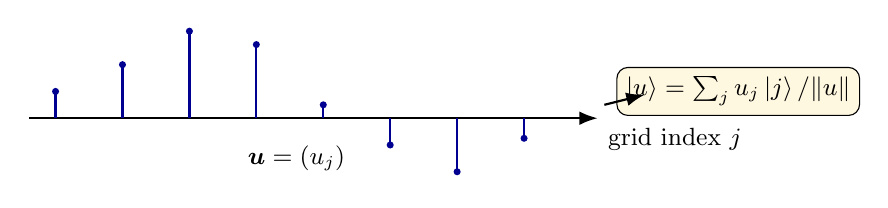
\begin{tikzpicture}[every node/.style={font=\small,align=center},scale=0.85]
\draw[-Latex,thick] (0,0)--(8.5,0) node[below right] {grid index $j$};
\foreach \x/\h in {0/0.4,1/0.8,2/1.3,3/1.1,4/0.2,5/-0.4,6/-0.8,7/-0.3}
{\draw[navy,thick] (\x+0.4,0)--(\x+0.4,\h); \fill[navy] (\x+0.4,\h) circle (1.5pt);}
\node at (4,-0.6) {$\bm u=(u_j)$};
\node[draw,rounded corners,fill=softyellow,align=center] at (10.6,0.4) {$\ket u=\sum_j u_j\ket j/\|u\|$};
\draw[-Latex,thick] (8.6,0.2)--(9.2,0.35);
\end{tikzpicture}
\end{center}
\begin{keybox}{量子算法输出}
最终态常为 $\ket{u(t)}$ 或其近似。若只需估计 $\langle u(t)|M|u(t)\rangle$，可能避免完全读出。
\end{keybox}
\end{frame}

\section{测量、估计与误差}

\begin{frame}{测量次数：一次运行通常不够}
若要估计 Bernoulli 随机变量 $X\in\{0,1\}$ 的均值 $p$，独立重复 $S$ 次，样本均值 $\hat p$ 满足
\[
\Pr(|\hat p-p|\ge \eps)\le 2e^{-2S\eps^2}.
\]
因此为了常数置信度达到加性误差 $\eps$，通常需要
\[
S=O(1/\eps^2)
\]
次 shots。
\begin{warnbox}{与量子线路复杂度相乘}
总成本往往是
\[
\text{总成本}=\text{单次线路成本}\times\text{shots 或 amplitude estimation 成本}.
\]
\end{warnbox}
\end{frame}

\begin{frame}{Hadamard test：估计 $\mathrm{Re}\bra\psi U\ket\psi$}
\begin{columns}[T,totalwidth=\textwidth]
\column{0.47\textwidth}
\begin{center}
\begin{quantikz}[row sep=0.30cm,column sep=0.42cm]
\lstick{$\ket0$} & \gate{H} & \ctrl{1} & \gate{H} & \meter{} \\
\lstick{$\ket\psi$} & \qw & \gate{U} & \qw & \qw
\end{quantikz}
\end{center}
测得辅助 qubit 为 $0$ 的概率为
\[
P(0)=\frac12\left(1+\mathrm{Re}\bra\psi U\ket\psi\right).
\]
\column{0.51\textwidth}
\begin{keybox}{推导}
受控 $U$ 后状态为
\[
\frac{1}{\sqrt2}(\ket0\ket\psi+\ket1U\ket\psi).
\]
再作用 $H$，辅助为 $0$ 的分量是
\[
\frac12\ket0(I+U)\ket\psi.
\]
其概率为
\[
\frac14\|(I+U)\ket\psi\|^2=\frac12(1+\mathrm{Re}\bra\psi U\ket\psi).
\]
\end{keybox}
\end{columns}
\end{frame}

\begin{frame}{Hadamard test 的虚部与一般内积}
\begin{keybox}{估计虚部}
在最后一个 $H$ 前给辅助 qubit 加相位门，可得到
\[
P(0)=\frac12\left(1+\mathrm{Im}\bra\psi U\ket\psi\right)
\]
或对应符号版本，取决于 $S/S^{\dagger}$ 的约定。
\end{keybox}
\begin{exbox}{一般内积}
若可制备 $\ket u=A\ket0$ 和 $\ket v=B\ket0$，则
\[
\braket{u|v}=\bra0 A^{\dagger}B\ket0.
\]
令 $U=A^{\dagger}B$，Hadamard test 可估计 $\braket{u|v}$ 的实部与虚部。
\end{exbox}
\end{frame}

\begin{frame}{SWAP test：估计 $|\braket{u|v}|^2$}
\begin{columns}[T,totalwidth=\textwidth]
\column{0.50\textwidth}
\begin{center}
\begin{quantikz}[row sep=0.3cm,column sep=0.42cm]
\lstick{$\ket0$} & \gate{H} & \ctrl{1} & \gate{H} & \meter{} \\
\lstick{$\ket u$} & \qw & \swap{1} & \qw & \qw \\
\lstick{$\ket v$} & \qw & \targX{} & \qw & \qw
\end{quantikz}
\end{center}
\[
P(0)=\frac12\left(1+|\braket{u|v}|^2\right).
\]
\column{0.48\textwidth}
\begin{keybox}{推导核心}
线路最后测量辅助为 $0$ 对应未归一化状态
\[
\frac12(\ket u\ket v+\ket v\ket u).
\]
其范数平方为
\[
\frac14(2+2|\braket{u|v}|^2).
\]
故
\[
|\braket{u|v}|^2=2P(0)-1.
\]
\end{keybox}
\end{columns}
\begin{warnbox}{限制}
SWAP test 只能给出内积模平方，不能直接恢复相位。
\end{warnbox}
\end{frame}

\begin{frame}{Postselection：成功分支与概率损失}
许多量子子程序产生如下形式：
\[
U\ket0\ket\psi=\sqrt p\ket0\ket{\phi}+\sqrt{1-p}\ket{\perp}.
\]
若只接受辅助寄存器测量为 $0$ 的分支，则成功概率为 $p$。
\begin{columns}[T,totalwidth=\textwidth]
\column{0.5\textwidth}
\begin{keybox}{重复采样}
平均需要 $O(1/p)$ 次。
\end{keybox}
\column{0.5\textwidth}
\begin{keybox}{振幅放大}
若能实现反射，通常可降到 $O(1/\sqrt p)$ 次。
\end{keybox}
\end{columns}
\vspace{2mm}
\begin{warnbox}{科学计算中的常见风险}
若 $p$ 与条件数、归一化系数或时间指数相关，postselection 可能吞掉理论加速。
\end{warnbox}
\end{frame}

\begin{frame}{误差来源：量子算法要同时记账}
\begin{center}
\begin{tikzpicture}[node distance=7mm,every node/.style={font=\small,align=center}]
\node[draw,rounded corners,fill=softblue,minimum width=2.3cm,minimum height=0.75cm] (disc) {离散化误差};
\node[draw,rounded corners,fill=softgreen,right=of disc,minimum width=2.3cm,minimum height=0.75cm] (prep) {初态制备误差};
\node[draw,rounded corners,fill=softyellow,right=of prep,minimum width=2.3cm,minimum height=0.75cm] (alg) {线路近似误差};
\node[draw,rounded corners,fill=softred,right=of alg,minimum width=2.3cm,minimum height=0.75cm] (shot) {采样误差};
\draw[-Latex,thick] (disc)--(prep); \draw[-Latex,thick] (prep)--(alg); \draw[-Latex,thick] (alg)--(shot);
\end{tikzpicture}
\end{center}
\begin{keybox}{hybrid argument}
若每一步酉近似满足 $\|U_j-V_j\|\le\delta_j$，则
\[
\left\|U_m\cdots U_1-V_m\cdots V_1\right\|
\le \sum_{j=1}^m\delta_j.
\]
\end{keybox}
\begin{exbox}{证明一行}
插入望远镜和酉范数不变性：
\[
U_m\cdots U_1-V_m\cdots V_1=\sum_j V_m\cdots V_{j+1}(U_j-V_j)U_{j-1}\cdots U_1.
\]
\end{exbox}
\end{frame}

\begin{frame}{量子复杂度：三种常用指标}
\begin{center}
\renewcommand{\arraystretch}{1.2}
\begin{tabular}{p{0.25\textwidth}p{0.60\textwidth}}
\toprule
指标 & 含义\\
\midrule
qubit complexity & 逻辑 qubit 数，包括系统寄存器、辅助寄存器、相位寄存器、oracle 工作空间\\
gate complexity & 基本逻辑门数，尤其是 $T$ 门数和受控操作成本\\
query complexity & 对黑盒 oracle、block-encoding 或 state-preparation unitary 的调用次数\\
shot complexity & 为估计概率或期望值所需重复运行次数\\
classical preprocessing & 离散化、构造数据结构、参数计算、编译等经典成本\\
\bottomrule
\end{tabular}
\end{center}
\begin{warnbox}{避免“只报 query complexity”}
对数学算法有启发意义，但实际课程中要说明 query、gate、qubit、shot 与经典预处理分别是什么。
\end{warnbox}
\end{frame}

\section{矩阵、Hamiltonian 与科学计算接口}

\begin{frame}{谱定理、SVD 与矩阵函数：量子算法的共同语言}
\begin{columns}[T,totalwidth=\textwidth]
\column{0.5\textwidth}
\begin{keybox}{Hermitian 矩阵}
若 $A=A^{\dagger}$，则
\[
A=\sum_j \lambda_j\ket{v_j}\bra{v_j},
\quad f(A)=\sum_j f(\lambda_j)\ket{v_j}\bra{v_j}.
\]
\end{keybox}
\column{0.5\textwidth}
\begin{keybox}{一般矩阵}
若 $A=\sum_j \sigma_j\ket{u_j}\bra{v_j}$，则奇异值变换关注
\[
f^{(SV)}(A)=\sum_j f(\sigma_j)\ket{u_j}\bra{v_j}.
\]
\end{keybox}
\end{columns}
\vspace{2mm}
\begin{exbox}{算法例子}
Hamiltonian simulation 实现 $e^{-iHt}$；线性系统求解希望实现 $A^{-1}$；QSVT 则把多项式函数作用到奇异值上。
\end{exbox}
\end{frame}


\begin{frame}{稀疏矩阵：从数学矩阵到 oracle 访问}
\small
$d$-sparse 矩阵 $A\in\mathbb C^{N\times N}$ 表示每行最多 $d$ 个非零元。常用 oracle 形式为
\[
O_{\rm loc}:\ket{i,k}\mapsto\ket{i,\ell(i,k)},
\qquad
O_{\rm val}:\ket{i,j,0}\mapsto\ket{i,j,A_{ij}}.
\]
其中 $\ell(i,k)$ 是第 $i$ 行第 $k$ 个非零元的列号。
\begin{center}
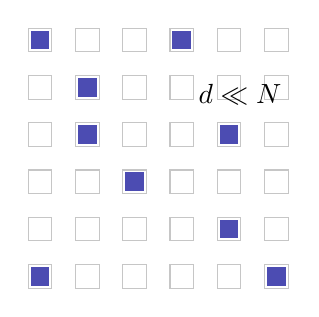
\begin{tikzpicture}[scale=0.60]
\foreach \i in {0,...,5}{\foreach \j in {0,...,5}{\draw[gray!45] (\j,-\i) rectangle +(0.5,-0.5);}}
\foreach \i/\j in {0/0,0/3,1/1,2/1,2/4,3/2,4/4,5/0,5/5}{\fill[navy!70] (\j+0.05,-\i-0.05) rectangle +(0.4,-0.4);}
\node[right] at (3.4,-1.4) {$d\ll N$};
\end{tikzpicture}
\end{center}
\begin{warnbox}{口径}
Oracle 的构造本身可能很贵；不能把任意大矩阵免费视为可查询对象。
\end{warnbox}
\end{frame}

\begin{frame}{优化问题的 Hamiltonian 表示：MaxCut 例子}
对图 $G=(V,E)$，MaxCut 可写为二进制优化
\[
\max_{z_i\in\{\pm1\}}\frac12\sum_{(i,j)\in E}(1-z_iz_j).
\]
量子表示中用 Pauli-$Z$ 的本征值对应 $z_i$：
\[
H_C=\frac12\sum_{(i,j)\in E}(I-Z_iZ_j).
\]
\begin{columns}[T,totalwidth=\textwidth]
\column{0.48\textwidth}
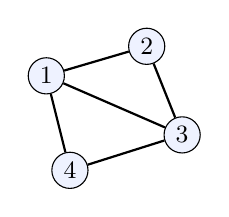
\begin{tikzpicture}[scale=0.75,every node/.style={circle,draw,fill=softblue,inner sep=2pt,font=\small}]
\node (1) at (0,1) {1}; \node (2) at (1.7,1.5) {2}; \node (3) at (2.3,0) {3}; \node (4) at (0.4,-0.6) {4};
\draw[thick] (1)--(2)--(3)--(4)--(1); \draw[thick] (1)--(3);
\end{tikzpicture}
\column{0.5\textwidth}
\begin{keybox}{矩阵观点}
$H_C$ 在计算基下是对角矩阵，每个 bit string 的能量等于对应 cut value。
\end{keybox}
\end{columns}
\end{frame}

\begin{frame}{Pauli 分解：Hamiltonian 的线路入口}
$n$ qubit 上的 Pauli 字符串
\[
P=P_1\otimes\cdots\otimes P_n,
\qquad P_j\in\{I,X,Y,Z\}
\]
构成矩阵空间的一组正交基。任意 Hermitian 矩阵可写成
\[
H=\sum_{\ell} h_{\ell}P_{\ell},\qquad h_{\ell}\in\mathbb R.
\]
\begin{keybox}{为什么有用？}
若可以实现每个 $e^{-ih_{\ell}P_{\ell}t}$，则可用 Lie--Trotter、LCU、qubitization 等方法模拟 $e^{-iHt}$。
\end{keybox}
\begin{exbox}{单 Pauli 指数}
由于 $P^2=I$，
\[
e^{-i\theta P}=\cos\theta\,I-i\sin\theta\,P.
\]
\end{exbox}
\end{frame}

\section{QFT 与 QPE}

\begin{frame}{经典 DFT 与 QFT 的区别}
令 $N=2^n$，经典 DFT 把向量 $x=(x_0,\ldots,x_{N-1})$ 变为
\[
y_k=\frac1{\sqrt N}\sum_{j=0}^{N-1}\omega_N^{jk}x_j,
\quad \omega_N=e^{2\pi i/N}.
\]
QFT 是同一个酉矩阵，但作用对象是量子态：
\[
F_N:\ket{j}\mapsto \frac1{\sqrt N}\sum_{k=0}^{N-1}\omega_N^{jk}\ket{k}.
\]
\begin{warnbox}{不要混淆}
QFT 不会把一个经典数组的所有 Fourier 系数一次性输出；它把量子态的振幅做 Fourier 变换，测量仍然只能给出样本。
\end{warnbox}
\end{frame}

\begin{frame}{QFT 的酉性证明}
QFT 矩阵元为
\[
(F_N)_{k,j}=\frac{1}{\sqrt N}\omega_N^{jk}.
\]
验证 $F_N^{\dagger}F_N=I$：
\[
(F_N^{\dagger}F_N)_{\ell,j}
=\frac1N\sum_{k=0}^{N-1}\omega_N^{k(j-\ell)}.
\]
若 $j=\ell$，和为 $1$；若 $j\ne \ell$，由几何级数
\[
\sum_{k=0}^{N-1}r^k=\frac{1-r^N}{1-r}=0,
\qquad r=\omega_N^{j-\ell}\ne1.
\]
所以
\[
(F_N^{\dagger}F_N)_{\ell,j}=\delta_{\ell j}.
\]
\end{frame}

\begin{frame}{QFT product form：二进制小数}
设 $j=(j_{n-1}\cdots j_0)_2$。定义二进制小数
\[
0.j_rj_{r-1}\cdots j_0=\sum_{s=0}^{r}j_s2^{s-r-1}.
\]
则 QFT 有分解
\[
F_{2^n}\ket{j}=\frac{1}{2^{n/2}}\bigotimes_{r=0}^{n-1}
\left(\ket0+e^{2\pi i\,0.j_rj_{r-1}\cdots j_0}\ket1\right)
\]
（通常还伴随输出 qubit 顺序反转）。
\begin{keybox}{意义}
这个乘积形式解释了为什么 QFT 可用 $O(n^2)$ 个 Hadamard 与受控相位门实现，而不是 $O(N^2)$。
\end{keybox}
\end{frame}

\begin{frame}{QFT 线路：Hadamard、受控相位与 SWAP}
\begin{center}
\begin{quantikz}[row sep=0.28cm,column sep=0.35cm]
\lstick{$q_2$} & \gate{H} & \ctrl{1} & \ctrl{2} & \qw      & \qw      & \swap{2} & \qw \\
\lstick{$q_1$} & \qw      & \gate{R_2} & \qw & \gate{H} & \ctrl{1} & \qw      & \qw \\
\lstick{$q_0$} & \qw      & \qw      & \gate{R_3} & \qw & \gate{R_2} & \targX{} & \qw
\end{quantikz}
\end{center}
其中
\[
R_m=\begin{pmatrix}1&0\\0&e^{2\pi i/2^m}\end{pmatrix}.
\]
\begin{keybox}{门复杂度}
精确 QFT 需要 $O(n^2)$ 个基本受控相位门；若忽略角度很小的旋转，可得到 approximate QFT，复杂度约 $O(n\log(n/\eps))$。
\end{keybox}
\end{frame}

\begin{frame}{QPE 问题设置：估计酉矩阵本征相位}
给定酉矩阵 $U$ 和其本征态 $\ket\psi$：
\[
U\ket\psi=e^{2\pi i\varphi}\ket\psi,
\qquad \varphi\in[0,1).
\]
Quantum Phase Estimation 目标是估计 $\varphi$ 的二进制展开。
\begin{center}
\begin{tikzpicture}[node distance=8mm,every node/.style={font=\small,align=center}]
\node[draw,rounded corners,fill=softblue,minimum width=2.6cm,minimum height=0.8cm] (in) {$\ket0^{\otimes m}\ket\psi$};
\node[draw,rounded corners,fill=softyellow,right=of in,minimum width=2.8cm,minimum height=0.8cm] (powers) {controlled $U^{2^r}$};
\node[draw,rounded corners,fill=softgreen,right=of powers,minimum width=2.6cm,minimum height=0.8cm] (iqft) {inverse QFT};
\node[draw,rounded corners,fill=softred,right=of iqft,minimum width=2.6cm,minimum height=0.8cm] (meas) {测量 $\tilde\varphi$};
\draw[-Latex,thick] (in)--(powers); \draw[-Latex,thick] (powers)--(iqft); \draw[-Latex,thick] (iqft)--(meas);
\end{tikzpicture}
\end{center}
\begin{keybox}{为什么重要？}
QPE 是 Shor 算法、Hamiltonian eigenvalue estimation、HHL 与许多早期量子线性代数算法的核心子程序。
\end{keybox}
\end{frame}

\begin{frame}{QPE 线路结构}
\begin{center}
\begin{quantikz}[row sep=0.26cm,column sep=0.32cm]
\lstick{$\ket0$} & \gate{H} & \ctrl{3} & \qw      & \qw      & \qw & \gate[wires=3]{F_{2^m}^{\dagger}} & \meter{} \\
\lstick{$\ket0$} & \gate{H} & \qw      & \ctrl{2} & \qw      & \qw &                                         & \meter{} \\
\lstick{$\ket0$} & \gate{H} & \qw      & \qw      & \ctrl{1} & \qw &                                         & \meter{} \\
\lstick{$\ket\psi$} & \qw & \gate{U^{2^{m-1}}} & \gate{U^{2^{m-2}}} & \gate{U} & \qw & \qw & \qw
\end{quantikz}
\end{center}
\begin{keybox}{相位寄存器长度}
$m$ 个相位 qubit 给出 $M=2^m$ 个可能输出，精度尺度为 $O(1/M)$。
\end{keybox}
\end{frame}

\begin{frame}{QPE 第一步：Hadamard 产生均匀叠加}
相位寄存器初态为 $\ket0^{\otimes m}$。作用 $H^{\otimes m}$ 得到
\[
\ket0^{\otimes m}\mapsto \frac1{\sqrt M}\sum_{j=0}^{M-1}\ket j,
\qquad M=2^m.
\]
整体状态为
\[
\frac1{\sqrt M}\sum_{j=0}^{M-1}\ket j\ket\psi.
\]
\begin{exbox}{数学直觉}
相位寄存器枚举所有幂次 $j$；后续 controlled powers 会把本征相位写入 $\ket j$ 的相位因子。
\end{exbox}
\end{frame}

\begin{frame}{QPE 第二步：相位回踢}
受控幂次作用后
\[
\ket j\ket\psi\mapsto \ket j U^j\ket\psi.
\]
若 $U\ket\psi=e^{2\pi i\varphi}\ket\psi$，则
\[
U^j\ket\psi=e^{2\pi ij\varphi}\ket\psi.
\]
因此整体态变为
\[
\frac1{\sqrt M}\sum_{j=0}^{M-1}e^{2\pi ij\varphi}\ket j\ket\psi.
\]
\begin{keybox}{本质}
本征相位从目标寄存器“回踢”到了相位寄存器的 Fourier 态中。
\end{keybox}
\end{frame}

\begin{frame}{QPE 第三步：精确二进制相位情形}
若 $\varphi=a/M$，其中 $a\in\{0,\ldots,M-1\}$，则
\[
\frac1{\sqrt M}\sum_{j=0}^{M-1}e^{2\pi ija/M}\ket j=F_M\ket a.
\]
作用 $F_M^{\dagger}$ 后得到
\[
\ket a.
\]
于是测量相位寄存器精确输出 $a$，从而
\[
\tilde\varphi=\frac{a}{M}.
\]
\begin{exbox}{例}
$m=3$，若 $\varphi=5/8=0.101_2$，QPE 输出 bit string $101$。
\end{exbox}
\end{frame}

\begin{frame}{一般相位：为什么输出集中在 $M\varphi$ 附近？}
对任意 $\varphi$，测量到 $a$ 的振幅为
\[
\frac1M\sum_{j=0}^{M-1}e^{2\pi ij(\varphi-a/M)}.
\]
概率为
\[
P(a)=\frac1{M^2}\left|\frac{1-e^{2\pi iM(\varphi-a/M)}}{1-e^{2\pi i(\varphi-a/M)}}\right|^2.
\]
这是一个离散 Dirichlet kernel，峰值集中在 $a\approx M\varphi$ 附近。
\begin{keybox}{精度-成功概率}
通过增加相位 qubit 数和少量冗余位，可使估计误差达到 $\eps$ 且失败概率不超过 $\delta$，典型相位 qubit 数为 $O(\log(1/\eps)+\log(1/\delta))$。
\end{keybox}
\end{frame}

\begin{frame}{一个具体例子：$M=8,\;\varphi=0.30$}
$M\varphi=2.4$，输出应集中在 $a=2$ 或 $a=3$ 附近。
\begin{center}
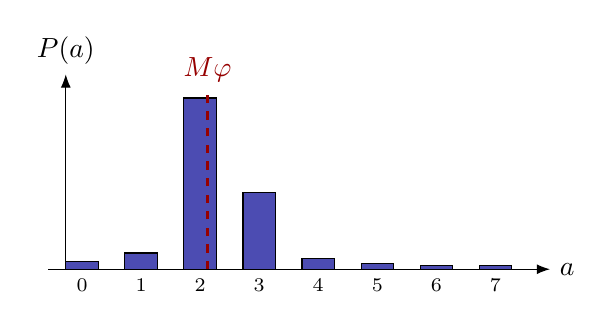
\begin{tikzpicture}[scale=0.75]
\foreach \a/\p in {0/0.025,1/0.055,2/0.58,3/0.26,4/0.035,5/0.018,6/0.014,7/0.013}{
  \draw[fill=navy!70] (\a,0) rectangle +(0.55,{5*\p});
  \node[below] at (\a+0.275,0) {\scriptsize \a};
}
\draw[-Latex] (-0.3,0)--(8.2,0) node[right] {$a$};
\draw[-Latex] (0,0)--(0,3.3) node[above] {$P(a)$};
\draw[deepred,thick,dashed] (2.4,0)--(2.4,3.0) node[above] {$M\varphi$};
\end{tikzpicture}
\end{center}
\begin{warnbox}{读图}
QPE 不是求连续相位的神谕；它通过有限相位寄存器得到一个离散分布，精度由 $m$ 决定。
\end{warnbox}
\end{frame}

\begin{frame}{若输入不是本征态}
若
\[
\ket b=\sum_k c_k\ket{\psi_k},
\qquad U\ket{\psi_k}=e^{2\pi i\varphi_k}\ket{\psi_k},
\]
则 QPE 线性作用后得到近似
\[
\sum_k c_k\ket{\widetilde{\varphi_k}}\ket{\psi_k}.
\]
测量相位寄存器会以约 $|c_k|^2$ 的概率抽到对应本征相位。
\begin{keybox}{与线性代数的关系}
QPE 相当于把输入态按 $U$ 的本征基展开，并把本征值信息写入辅助寄存器。HHL 正是利用这一点对不同特征值分量施加不同旋转。
\end{keybox}
\end{frame}

\begin{frame}{QPE 与 Hamiltonian 特征值估计}
若 $H\ket{v_k}=\lambda_k\ket{v_k}$，令
\[
U=e^{-iHt}.
\]
则
\[
U\ket{v_k}=e^{-i\lambda_k t}\ket{v_k}=e^{2\pi i\varphi_k}\ket{v_k}.
\]
因此 QPE 可估计 $\lambda_k$ modulo $2\pi/t$：
\[
\lambda_k\approx -\frac{2\pi}{t}\varphi_k.
\]
\begin{warnbox}{两个技术点}
\begin{itemize}
\item 需要可实现 $e^{-iHt}$ 及其受控幂次。
\item 需要选择 $t$ 避免谱 aliasing，并处理正负特征值映射。
\end{itemize}
\end{warnbox}
\end{frame}

\begin{frame}{QPE 小结：它为什么是 QFT 的应用？}
\begin{center}
\begin{tikzpicture}[node distance=7mm,every node/.style={font=\small,align=center}]
\node[draw,rounded corners,fill=softblue,minimum width=3cm,minimum height=0.75cm] (phase) {相位函数\\$j\mapsto e^{2\pi ij\varphi}$};
\node[draw,rounded corners,fill=softyellow,right=of phase,minimum width=3cm,minimum height=0.75cm] (fourier) {Fourier 态\\$F_M\ket{a}$};
\node[draw,rounded corners,fill=softgreen,right=of fourier,minimum width=3cm,minimum height=0.75cm] (bits) {逆 QFT\\输出二进制 $a$};
\draw[-Latex,thick] (phase)--(fourier); \draw[-Latex,thick] (fourier)--(bits);
\end{tikzpicture}
\end{center}
\begin{keybox}{一句话}
QPE 先把本征相位变成相位寄存器上的周期振荡，再用 inverse QFT 把频率转换成二进制数字。
\end{keybox}
\end{frame}

\section{基础算法图景}

\begin{frame}{Deutsch--Jozsa：干涉如何给出全局信息}
给定 $f:\{0,1\}^n\to\{0,1\}$，承诺 $f$ 要么常数，要么平衡。oracle 为
\[
U_f\ket{x}\ket y=\ket{x}\ket{y\oplus f(x)}.
\]
取目标 qubit 为 $\ket-=(\ket0-\ket1)/\sqrt2$，有相位 oracle：
\[
U_f\ket{x}\ket-=(-1)^{f(x)}\ket{x}\ket-.
\]
\begin{keybox}{判别量}
对输入寄存器做 $H^{\otimes n}$、oracle、再 $H^{\otimes n}$，测到 $0^n$ 的振幅为
\[
\frac1{2^n}\sum_x(-1)^{f(x)}.
\]
常数函数给 $\pm1$，平衡函数给 $0$。
\end{keybox}
\end{frame}

\begin{frame}{Grover 搜索：二维旋转图像}
目标集合 $G$，好态比例 $a=|G|/N$。令
\[
\ket{g}=\frac1{\sqrt{|G|}}\sum_{x\in G}\ket x,
\quad
\ket{b}=\frac1{\sqrt{N-|G|}}\sum_{x\notin G}\ket x.
\]
均匀叠加为
\[
\ket s=\sqrt a\ket g+\sqrt{1-a}\ket b.
\]
Grover 迭代由 oracle 反射和关于 $\ket s$ 的反射组成，在 $\mathrm{span}\{\ket g,\ket b\}$ 中每次旋转约 $2\theta$，其中 $\sin^2\theta=a$。
\begin{center}
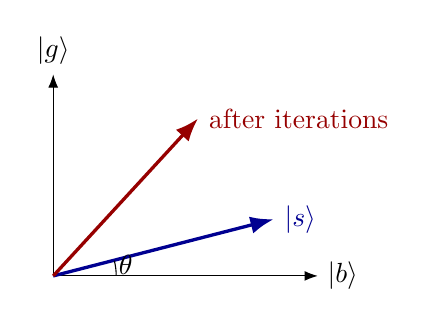
\begin{tikzpicture}[scale=0.8]
\draw[-Latex] (0,0)--(4.2,0) node[right] {$\ket b$};
\draw[-Latex] (0,0)--(0,3.2) node[above] {$\ket g$};
\draw[navy,very thick,-Latex] (0,0)--(3.5,0.9) node[right] {$\ket s$};
\draw[deepred,very thick,-Latex] (0,0)--(2.3,2.5) node[right] {after iterations};
\draw (1,0) arc (0:14:1); \node at (1.15,0.17) {$\theta$};
\end{tikzpicture}
\end{center}
\end{frame}

\begin{frame}{Amplitude amplification：Grover 的抽象版本}
设算法 $A$ 满足
\[
A\ket0=\sqrt a\ket{\mathrm{good}}+\sqrt{1-a}\ket{\mathrm{bad}}.
\]
若直接重复，期望 $O(1/a)$ 次才成功。振幅放大通过两个反射
\[
S_0=I-2\ket0\bra0,
\qquad S_{\chi}=I-2\Pi_{\mathrm{good}},
\]
构造
\[
Q=-A S_0 A^{\dagger}S_{\chi},
\]
把成功概率提升到常数，只需 $O(1/\sqrt a)$ 次调用。
\begin{warnbox}{必须能用 $A^{\dagger}$}
振幅放大不是黑盒重复；它需要算法 $A$ 无中途测量且可逆实现，以便使用逆线路。
\end{warnbox}
\end{frame}

\begin{frame}{Shor 算法在基础课中的位置}
Shor 分解的量子部分可视为“找周期”：
\[
f(x)=a^x\bmod N.
\]
通过周期态、QFT 与 continued fractions 估计周期 $r$，再由数论恢复因子。
\begin{center}
\begin{tikzpicture}[node distance=7mm,every node/.style={font=\small,align=center}]
\node[draw,rounded corners,fill=softblue] (num) {数论化简};
\node[draw,rounded corners,fill=softyellow,right=of num] (q) {量子找周期};
\node[draw,rounded corners,fill=softgreen,right=of q] (cf) {连分数恢复 $r$};
\node[draw,rounded corners,fill=softred,right=of cf] (fac) {求因子};
\draw[-Latex,thick] (num)--(q); \draw[-Latex,thick] (q)--(cf); \draw[-Latex,thick] (cf)--(fac);
\end{tikzpicture}
\end{center}
\begin{keybox}{本课只需记住}
Shor 算法证明 QFT/QPE 不只是形式工具，而能产生超多项式量子加速；后续科学计算算法也大量复用相位估计思想。
\end{keybox}
\end{frame}

\section{PDE 与 Fourier 谱方法接口}

\begin{frame}{周期问题为什么适合 Fourier 谱方法？}
周期函数可展开为
\[
u(x)=\sum_{k\in\mathbb Z}\hat u_k e^{ikx}.
\]
微分变成频率侧乘法：
\[
\partial_x u \longleftrightarrow ik\hat u_k,
\qquad
\partial_{xx}u \longleftrightarrow -k^2\hat u_k.
\]
\begin{keybox}{量子接口}
QFT 正好在网格态上实现离散 Fourier 变换；如果 PDE 在 Fourier 侧对角化，就可把演化化为相位门或对角操作。
\end{keybox}
\end{frame}

\begin{frame}{离散 Fourier 变换：从网格值到频率系数}
令 $u_j=u(x_j)$，$j=0,\ldots,N-1$。定义
\[
\tilde u_k=\frac1{\sqrt N}\sum_{j=0}^{N-1}u_j e^{-2\pi ijk/N},
\qquad
u_j=\frac1{\sqrt N}\sum_{k=0}^{N-1}\tilde u_k e^{2\pi ijk/N}.
\]
离散 Parseval 恒等式为
\[
\sum_j |u_j|^2=\sum_k |\tilde u_k|^2.
\]
\begin{warnbox}{符号约定}
经典 DFT 与 QFT 可能在指数正负号、归一化、频率排序上不同。PDE 推导中必须固定约定，尤其是 Laplacian symbol 的符号。
\end{warnbox}
\end{frame}

\begin{frame}{谱微分：DFT - 乘 symbol - IDFT}
对周期网格函数，谱微分可写为
\[
D_x = F_N^{\dagger}\,\mathrm{diag}(ik)\,F_N,
\]
二阶导数为
\[
D_{xx}=F_N^{\dagger}\,\mathrm{diag}(-k^2)\,F_N.
\]
\begin{center}
\begin{tikzpicture}[node distance=7mm,every node/.style={font=\small,align=center}]
\node[draw,rounded corners,fill=softblue] (u) {网格值 $u_j$};
\node[draw,rounded corners,fill=softyellow,right=of u] (F) {DFT/QFT};
\node[draw,rounded corners,fill=softgreen,right=of F] (sym) {乘 $ik$ 或 $-k^2$};
\node[draw,rounded corners,fill=softred,right=of sym] (Finv) {IDFT/IQFT};
\node[draw,rounded corners,fill=white,right=of Finv] (du) {导数值};
\draw[-Latex,thick] (u)--(F); \draw[-Latex,thick] (F)--(sym); \draw[-Latex,thick] (sym)--(Finv); \draw[-Latex,thick] (Finv)--(du);
\end{tikzpicture}
\end{center}
\end{frame}

\begin{frame}{周期 Schr\"odinger 方程：第一个完整例子}
考虑
\[
i\partial_t u(x,t)=-\Delta u(x,t),
\qquad x\in[0,2\pi]^d.
\]
Fourier 系数满足
\[
i\frac{d}{dt}\hat u_k(t)=|k|^2\hat u_k(t),
\]
因此
\[
\hat u_k(t)=e^{-i|k|^2t}\hat u_k(0).
\]
\begin{keybox}{量子线路思路}
\[
\ket{u(0)}\xrightarrow{QFT}\sum_k \hat u_k(0)\ket k
\xrightarrow{\mathrm{phase}}\sum_k e^{-i|k|^2t}\hat u_k(0)\ket k
\xrightarrow{QFT^{\dagger}}\ket{u(t)}.
\]
\end{keybox}
\end{frame}

\begin{frame}{从经典谱方法到量子谱方法}
\begin{center}
\begin{tikzpicture}[node distance=7mm,every node/.style={font=\small,align=center}]
\node[draw,rounded corners,fill=softblue,minimum width=2.6cm] (classical) {经典数组 $u_j$};
\node[draw,rounded corners,fill=softyellow,right=of classical,minimum width=2.6cm] (fft) {FFT};
\node[draw,rounded corners,fill=softgreen,right=of fft,minimum width=2.6cm] (diag) {频率侧乘法};
\node[draw,rounded corners,fill=softred,right=of diag,minimum width=2.6cm] (ifft) {IFFT};
\draw[-Latex,thick] (classical)--(fft); \draw[-Latex,thick] (fft)--(diag); \draw[-Latex,thick] (diag)--(ifft);
\node[draw,rounded corners,fill=softblue,minimum width=2.6cm,below=1.0cm of classical] (qstate) {量子态 $\ket u$};
\node[draw,rounded corners,fill=softyellow,right=of qstate,minimum width=2.6cm] (qft) {QFT};
\node[draw,rounded corners,fill=softgreen,right=of qft,minimum width=2.6cm] (phase) {相位模块};
\node[draw,rounded corners,fill=softred,right=of phase,minimum width=2.6cm] (iqft) {IQFT};
\draw[-Latex,thick] (qstate)--(qft); \draw[-Latex,thick] (qft)--(phase); \draw[-Latex,thick] (phase)--(iqft);
\end{tikzpicture}
\end{center}
\begin{warnbox}{关键差别}
经典 FFT 输出完整频率数组；量子 QFT 输出的是量子态。若最终要全部网格值，量子优势通常消失。
\end{warnbox}
\end{frame}

\begin{frame}{PDE 量子算法的误差分解}
以周期 Schr\"odinger 方程为例，最终误差可分为
\[
\|u(t)-\tilde u_{\rm q}(t)\|
\le E_{\rm spectral}+E_{\rm stateprep}+E_{\rm QFT}+E_{\rm phase}+E_{\rm meas}.
\]
\begin{columns}[T,totalwidth=\textwidth]
\column{0.49\textwidth}
\begin{keybox}{数学误差}
\begin{itemize}
\item Fourier 截断误差
\item aliasing 或网格误差
\item 时间演化近似误差
\end{itemize}
\end{keybox}
\column{0.49\textwidth}
\begin{keybox}{量子误差}
\begin{itemize}
\item 初态制备误差
\item QFT/相位模块编译误差
\item 测量统计误差
\end{itemize}
\end{keybox}
\end{columns}
\end{frame}

\begin{frame}{何时可能有量子优势？}
\begin{keybox}{比较口径}
若网格点数 $N=2^n$，QFT 在门数上为 $\poly(n)$，经典 FFT 为 $O(N\log N)$。但这不自动意味着指数优势，因为还要计算：
\begin{itemize}
\item 制备 $\ket{u(0)}$ 的成本；
\item 频率相位 $e^{-i|k|^2t}$ 的可逆计算成本；
\item 需要读出的输出类型；
\item 与经典随机采样、低秩、稀疏、快速多极等最强算法的比较。
\end{itemize}
\end{keybox}
\begin{warnbox}{有希望的任务类型}
估计少量全局 observables、抽样、内积、能量、频率统计，而不是完整重构解向量。
\end{warnbox}
\end{frame}

\section{总结与阅读}

\begin{frame}{本课总结：从数学到量子算法}
\begin{enumerate}
\item 量子态是复 Hilbert 空间中的单位向量；复合系统由张量积给出。
\item 封闭演化是酉的，Hamiltonian 通过 $e^{-iHt}$ 生成酉演化。
\item 测量遵循 Born 规则，输出是随机样本；估计期望值需要 shots。
\item 线路模型把酉矩阵分解为基本门；可逆计算和 uncompute 至关重要。
\item QFT 是 DFT 的量子态版本；QPE 用 inverse QFT 读出本征相位。
\item PDE 量子算法必须同时说明离散化、编码、矩阵访问、输出与误差。
\end{enumerate}
\end{frame}

\begin{frame}{资料来源与阅读建议}
\footnotesize
\begin{thebibliography}{9}
\bibitem{NC} M. A. Nielsen and I. L. Chuang, \emph{Quantum Computation and Quantum Information}, Cambridge University Press, 10th Anniversary Edition, 2010.
\bibitem{Feynman} R. P. Feynman, ``Simulating physics with computers,'' \emph{International Journal of Theoretical Physics}, 21, 467--488, 1982.
\bibitem{Shor} P. W. Shor, ``Polynomial-Time Algorithms for Prime Factorization and Discrete Logarithms on a Quantum Computer,'' SIAM J. Comput., 26(5), 1484--1509, 1997.
\bibitem{Grover} L. K. Grover, ``A fast quantum mechanical algorithm for database search,'' STOC 1996 / arXiv:quant-ph/9605043.
\bibitem{BHMT} G. Brassard, P. Hoyer, M. Mosca, A. Tapp, ``Quantum Amplitude Amplification and Estimation,'' Contemporary Mathematics 305, 2002.
\bibitem{Lloyd} S. Lloyd, ``Universal quantum simulators,'' Science 273, 1073--1078, 1996.
\bibitem{IBM} IBM Quantum Documentation: Quantum Fourier Transform and Quantum Phase Estimation learning materials.
\end{thebibliography}
\end{frame}

\end{document}
